\documentclass[12pt,letterpaper]{article}
\usepackage{times}
\usepackage{fullpage}
\usepackage{graphicx}
\usepackage{caption}
\usepackage{fancyhdr}
\usepackage{lastpage}
\usepackage{indentfirst}
\usepackage{wrapfig}
%\usepackage{picins}
\usepackage{alltt}
\usepackage{array}
\usepackage{siunitx}

\widowpenalty10000%
\clubpenalty10000%
\tolerance=1000

%
\newcommand{\problem}[1]{\begin{center}\section{\protect\rule{0pt}{1.1em}#1}\rhead{\sffamily\bfseries\thesection\hspace{0.5em}#1}\end{center}}
\renewcommand{\thesection}{Problem \Alph{section}:}
%\renewcommand{\sectionmark}[1]{\markright{foo #1}}
\newcommand{\verbfile}[1]{\begin{alltt}\input{#1}\end{alltt}}

\makeatletter
\renewcommand{\@seccntformat}[1]{\csname the#1\endcsname\hspace{0.5em}}

\addtolength{\headheight}{20pt}
\addtolength{\textheight}{10pt}


\lhead{}
\rhead{}
\lfoot{\sffamily\bfseries Nov.~7, 2015}
\cfoot{\sffamily\bfseries 2015 Mid-Atlantic Regional Programming Contest}
\rfoot{\sffamily\bfseries Page \thepage\ of \pageref{LastPage}}

\newenvironment{icompact}{
  \begin{list}{$\bullet$}{
    \parsep 0pt plus 1pt
    \partopsep 0pt plus 1pt
    \topsep 2pt plus 2pt minus 1pt
    \itemsep 0pt plus 1pt
    \parskip 0pt plus 2pt
    \leftmargin 0.3in}
       \raggedright}
  {\normalsize\end{list}}

\newcounter{ecount}
\newenvironment{ecompact}{
  \begin{list}{\arabic{ecount}}{\usecounter{ecount}
    \parsep 0pt plus 1pt
    \partopsep 0pt plus 1pt
    \topsep 2pt plus 2pt minus 1pt
    \itemsep 0pt plus 1pt
    \leftmargin 0.3in}
       \raggedright}
  {\normalsize\end{list}}


\pagestyle{fancy}

\begin{document}

{\sffamily
\bfseries
\Large 
\begin{center}
\protect\rule{0pt}{1.1em}2015 Mid-Atlantic Regional Programming Contest
%\\ Draft \today
\end{center}
}


This is a courtesy copy of the problem set for the
Mid-Atlantic Regional contest.  It is an abbreviated version of the
problem set provided to the teams. Omitted are several pages of rules
and explanations of the contest and judging environment.


\begin{center}
{\large\bf Important:} 
\end{center}

The creation of this problem set was a collaboration
among Regional Contests scheduled for November 7. These
contests will be starting at different times and taking place in
different time zones.

In deference to the later starting contests, we ask that you refrain
from emailing, blogging, posting, tweeting, or otherwise making any public
comments about this problem set until November 8.

~

\hrule

~

\textbf{And now, a word from the head judge}

Without a team of creative volunteers, there would be no problem set
for this contest each year.  It's not too early to start thinking
about the 2016 contest!

We do require that problem authors not be coaches of or otherwise
directly associated with a participating team. But if you are a team
coach and have a colleague who might be interested in contributing,
please drop a word to them. If you have a creative team member who
will be an alumnus or alumna next year, you might do the same.

Anyone interested in participating as a member of the authoring team
for 2016 can send their contact information to this year's head judge
for the region, Steven Zeil, at \texttt{zeil@cs.odu.edu}.

\hrule

~


\begin{center}
\begin{tabular}{|c|c|c|}
  \hline
{\bfseries Problem}&
{\bfseries Problem Name}&
{\bfseries Balloon Color}\\
\hline
\hline
A&
Positive Con Sequences &
Orange \\
\hline
B&
Refract Facts &
Green \\
\hline
C &
Hounded by Indecision &
Silver \\
\hline
D&
Avoiding an Arrrgument   &
Pink \\
\hline
E&
Kinfolk &
Red \\
\hline
F&
Of the Children &
Yellow \\
\hline
G&
Talking About Numbers &
Black \\
\hline
H &
The Scheming Gardener &
Purple \\
\hline
\end{tabular}
\end{center}

%%% Local Variables: 
%%% mode: latex
%%% End: 


\sisetup{group-separator={,}}

\clearpage
\problem{Positive Con Sequences}

%\begin{wrapfigure}{r}{0.5\linewidth}
%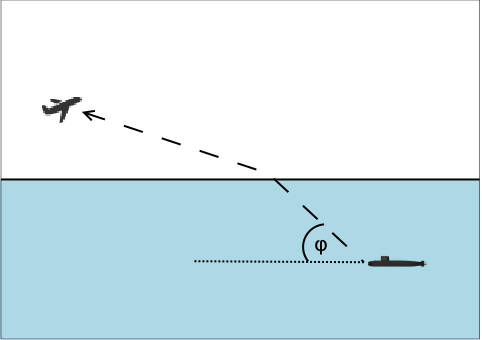
\includegraphics[width=\linewidth]{Refract/refract.png}
%\end{wrapfigure}

Your younger sister is studying for an upcoming standardized test in
mathematics, and needs practice with the common style of problem in
which the student is presented with a sequence of numbers with one
number missing and asked to fill in the missing value.

You are aware that the vast majority of these problems feature either
arithmetic sequences (where each number in the sequence is formed by
adding an integer constant to the prior number) or geometric sequences (where
each number in the sequence is formed by multiplying the prior number
by an integer constant).

Write a program that will help your sister drill on this style of
problem by allowing her to check her answers on sample problems.


\subsection*{Input}

Input will consist of one or more datasets.

Each dataset will be a single line containing $4$ integers defining a
sequence. One of these will be $-1$, denoting the missing value. The
remainder will be positive integers in the range $1\ldots \num{10000}$,
inclusive. Other than the $-1$ placeholder value, the values will be
in strictly increasing order.

End of input will be signaled by a line containing four $-1$
values.

\subsection*{Output}

For each dataset, print one line of output. 

If a positive integer in the range $1 \ldots \num{1000000}$ exists that
can be filled in to the missing value position to create an
arithmetic or geometric sequence, print that missing value. 

If there is no such positive integer, print -1.




\subsection*{Example}

Given the input:

\verbfile{Sequences/test0.in}


the output should be:

\verbfile{Sequences/test0.expected}



 
\clearpage
\problem{Refract Facts}

\begin{wrapfigure}{r}{0.5\linewidth}
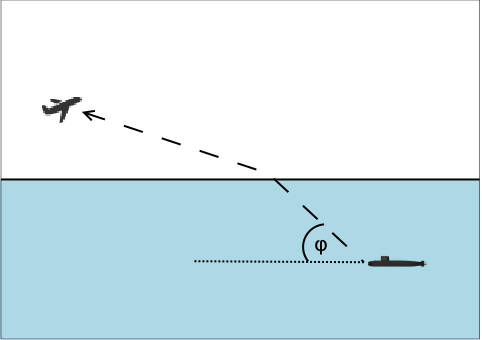
\includegraphics[width=\linewidth]{Refract/refract.png}
\end{wrapfigure}


A submarine is using a communications laser to send a message to a jet
cruising overhead.  The sea surface is flat. The submarine is cruising
at a depth $d$ below the surface. The jet is at height $h$ above the sea
surface, and a horizontal distance $x$ from the sub.  The submarine
turns toward the jet before starting communications, but needs to know
the angle of elevation, $\phi$, at which to aim the laser.

\begin{wrapfigure}{r}{0.5\linewidth}
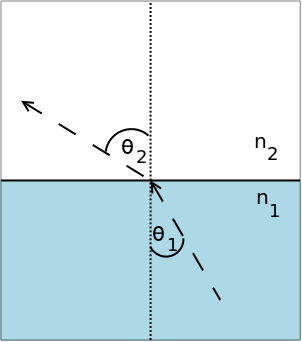
\includegraphics[width=\linewidth]{Refract/snell.png}
\end{wrapfigure}

When the laser passes from the sea into the air, it is refracted (its path is bent). The refraction is described by Snell's law, which says that light approaching the horizontal surface at an angle $\theta_1$, measured from the vertical, will leave at an angle $\theta_2$, given by the formula

\[ \frac{\sin \theta_1}{\sin \theta_2} = \frac{n_1}{n_2} \]

\noindent
where $n_1$ and $n_2$ are the respective {\em refraction indices} of
the water and air. (The refraction index of a material is inversely
proportional to how fast light can travel through that material.)

\subsection*{Input}

Input will consist of one or more datasets. 

Each dataset will consist of one line with 5 floating point
numbers. In order:

\begin{itemize}

\item $d$, the depth of the submarine (specifically, of the laser
  emitter) in feet, $1 \leq d \leq 800$

\item $h$, the height of the plane in feet, $100 \leq h \leq \num{10000}$

\item $x$, the horizontal distance from the sub to the plane in feet,
  $0 \leq x \leq \num{10000}$

\item $n_1$, the refractive index of water, $1.0 < n_1 \leq 2.5$, 

\item $n_2$, the refractive index of air, $1.0 \leq n_2 < n_1$ 
\end{itemize}

A value of 0 for $d$ will signal the end of input.

\subsection*{Output}

For each dataset, print a single line containing the angle of
elevation in degrees, to two decimals precision, at
which the submarine should aim its laser to illuminate the jet.




\subsection*{Example}

Given the input:

\verbfile{Refract/test0.in}


the output should be:

\verbfile{Refract/test0.expected}




\clearpage
\problem{Hounded by Indecision}

%\begin{wrapfigure}{r}{0.45\linewidth}
%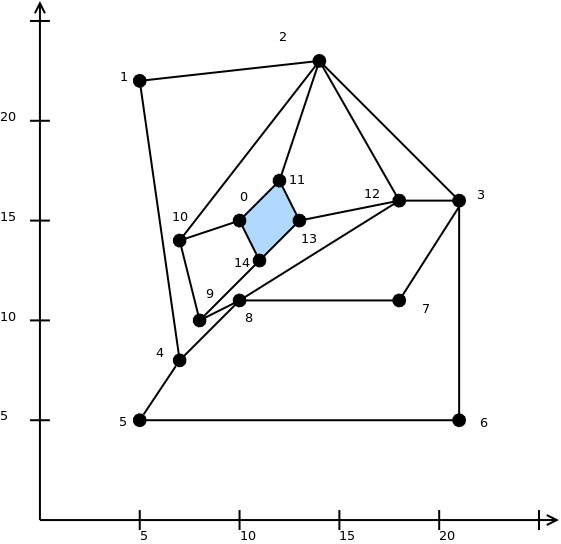
\includegraphics[width=\linewidth]{Gardener/plots1}
%\end{wrapfigure}

OK, maybe stealing the Duchess's favorite ruby necklace was not such a
good idea. You were making your way toward the city gates when you
heard the sound you had been dreading: a sharp whistle followed by an
answering bark. You know that the constable has just fetched his
favorite hound and is starting to search for you.  They might head
straight for a gate. They might try to pick up your trail on the
way. You really can't guess. But if they reach the gate before you,
you're caught. If they happen across your trail, the hound will pick
up your scent. The dog knows your scent already - this isn't your
first offense!  The constable will loose the hound, who can
run \textit{fast} once he has the trail to follow.

You have a dilemma. If you are absolutely sure that you can
reach the gates before the guard and before being overtaken by the
hound, you can keep the necklace. But if you aren't sure, you need to drop
the necklace right now into the nearest pile of rubbish and saunter
casually away. Even if they grab you, without the necklace in your
hands they will eventually release you.

So, keep the necklace or drop the necklace?

\hrulefill

The town is modeled as a rectangular maze of discrete squares.  It is
surrounded by a wall that contains one or more exits. You know, of
course, your own position within the town. You also know the location
of the kennel where the constable and the hound start out.

\begin{itemize}

\item In each turn (unit of time), you, the constable, and the hound 
move simultaneously. 

\item You can move zero or one square(s) horizontally or vertically per turn.

\item Initially, the constable and hound move together, also zero or 
one square(s) vertically or horizontally.

\item If the constable and the hound, moving together, reach a square
that you have previously occupied, the hound catches your scent and
the constable looses the hound. On each subsequent turn, the hound
follows your trail at a speed of one or two squares per turn. (The hound
moves two squares unless doing so would cause it to jump over the
thief or the exit.)

\item If the constable and/or the hound overtake you  (occupy the same
square as you), you are caught. To escape, you must reach an exit at
least one turn before the constable and/or hound.

\end{itemize}

\subsection*{Input}

Input consists of one or more mazes. Each maze begins with a line
containing two integers, $W$ and $H$, $3 \leq W,H \leq 40$, 
denoting the width and the height of
the maze. End of input is indicated when either of these values is
less than $3$.

This is followed by $H$ lines of input, each containing $W$
characters. 

The interpretation of the characters in these lines is as follows:

\begin{itemize}
\item ` ' denotes an open space

\item `K' is an open space denoting the kennel and hence the starting
position of the constable and the hound.  There will be exactly one of
these in any maze.

\item `T' is an open space denoting the original position of the thief
(you).  There will be exactly one of these in any maze.

\item `X' denotes a wall.

\item `E' is an open space representing an exit (a city gate). There will be at
least one of these. 

    All exits will occur on the outer perimeter (as defined by the W
    and H values) of the maze.

\end{itemize}


All mazes will be completely enclosed by a combination of `X' and `E'
characters.  There will be a path from the thief's starting location
to each exit and from the kennel to each exit.

\subsection*{Output}

For each maze, print a single line of output. If there is a path that
you can take that will guarantee that you can escape no matter what path
the constable and hound take, then print ``KEEP IT''.  If there is
no path that offers such a guarantee, print ``DROP IT''.






\subsection*{Example}

Given the input:

\clearpage
\verbfile{Hounded/test0.in}


the output should be:

\verbfile{Hounded/test0.expected}

In both cases, we can pretty much ignore the exit at the bottom of the
maze. The constable can always get there before the thief.

In the first case, if the thief heads straight for the exit on the
left, he emerges from the ``door'' on turn 4, and reaches the exit on
turn 11. On turn 7, the constable can reach the space where the thief
had been on turn 4, and would then loose the hound, which also reaches
the exit on turn 11, catching the thief.

In the second case, the thief has the option of taking the ``side
door'' out of the house, then heading for the wall before turning
right and heading for the exit. It's actually a longer path, taking 13
turns to reach the exit. But the constable won't reach the exit before
turn 14, and the earliest that the constable could
pick up the thief's trail would be on turn 11 (at the thief's staring
location), at which point the constable and hound are too far away to
catch the thief.

\clearpage
\problem{Avoiding an Arrrgument}

%\begin{wrapfigure}{r}{0.67\linewidth}
%\includegraphics[width=\linewidth]{Around/Row_Your_Boat.png}
%\end{wrapfigure}

The pirate captain and his crew gazed happily upon the chest brimming
with gemstones. Diamonds, rubies, sapphires, opals, and many other
kinds of gems added to the sparkling collection.

``We're rich, my lads!'' the captain said, ``Now, here's what we're
going to do. Each of us will take two stones now, then we'll bury the
rest because \ldots  because that's what pirates do!  Also, everyone
must take two different kinds of gems. We don't know what the merchants
in the next port will be buying, and I don't want to listen to any
belly-aching from someone who only took rubies if our next port
happens to have a flourishing ruby mine nearby''

``Who chooses first?'' asked the cabin boy, fearing that he already
knew the answer.

``I'll choose one first,'' said the captain, ``and then each man from
there in order of rank, starting with the first mate down to the cabin
boy''. The lower-ranked crew members began to grumble. ``Then,''
continued the captain, ``the cabin boy immediately chooses his second
gem, and we proceed in reversed order until we get to me, and I will
be the last to choose my second stone.''

The crew quickly agreed and, almost as quickly, began trying to figure
how to claim the best stones under this arrangement.

Write a program to figure out what stone a crewman should pick first
in order to maximize the total value they can be guaranteed to acquire
no matter how the rest of the crew chooses.


\subsection*{Input}

The input will consist of one or more data sets.

Each data set starts with a line containing 2 integers: $M$, the
number of kinds of gemstone available, and $N$, the number of crewmen
who select their first stone after you and select their second before
you.  Each data set will have $2 \leq M \leq 26$, $0 \leq N \leq 10$.
A value of 0 for $M$ indicates the end of input.

The remainder of the dataset consists of $M$ lines, each describing one
kind of available gem. The line begins with an uppercase alphabetic
character indicating the type of gem (e.g., 'D' might denote diamonds,
'Z' might stand for zircons). No two kinds of gem will have the same
code, but the codes may occur in any order.  The alphabetic code is
followed by $N+1$ integers, each demoting the value in doubloons of one
of the $N+1$ most valuable remaining gems of that kind. These will be
presented on the line in non-increasing order of value.  Values will
be in the range $0\ldots 10,000$.

\subsection*{Output}

For each dataset, print a single line containing the letter code for
the type of gem that you should pick first to maximize the total value
that you can be guaranteed to receive on both picks, no matter what
choices the rest of the crew makes.  If there is more than one type of
gem tied for the maximum total value, print the one the comes earliest
alphabetically.


\subsection*{Example}

Given the input:

\verbfile{Arrrgument/test0.in}


the output should be

\verbfile{Arrrgument/test0.expected}
 
\clearpage
\problem{Kinfolk}



The English language abounds with terms for describing family
(genetic) relationships.

The basic relationships are:

\begin{itemize}
\item ``Parent'' and ``child'' are well understood.

\item Children of the same parent are ``siblings''.

\item The child of your sibling is your niece (if she is female) or
  nephew (if he is male). You would be their aunt (if you are female)
  or uncle (if you are male).

\item Two people who share a common grandparent but not a common
  parent are ``1st cousins''.  If they share a common
  great-grandparent but not a common grandparent, they are ``2nd
  cousins''. This can be extended to ``3rd cousins'', ``4th cousins'',
  and so on.
\end{itemize}

These relationships are extended to later generations as follows:

\begin{itemize}

\item The ``child'', ``niece'', and ``nephew'' relationships can be extended
  to later generations by pre-pending ``grand'', ``great-grand'', or
  ``great-great-grand''.  Thus the child of one's child is a
  grandchild. The male child of your niece or nephew is your
  grandnephew. You grandnephew's female child would be your
  great-grandniece, and so on. (In theory, we could extend this to any
  number of additional ``great-'' prefixes, but we will stop with
  ``great-great-grand'' in this problem.)

\item The ``parent'', ``aunt'', and ``uncle'' relationships are extended
  symmetrically by the same prefix. Thus you would be the grandparent
  of your grandchild, the great-granduncle or great-grandaunt of your
  great-grandnieces and great-grandnephews, etc.

\item The ``cousin'' relationship is extended to your cousin's descendants
  by degrees of removal. The children of your 1st cousin are your
  first cousins once removed (and, symmetrically, you are their 1st
  cousin once removed).  The grand-children of your 3rd cousin are
  your 3rd cousins twice removed.The great-grandchildren of your 2nd
  cousin are your 2nd cousins thrice removed. All of the cousin-based
  relationships are symmetric, so if someone is your
  \textit{K}$^{\mbox{th}}$ cousin \textit{something} removed, you are
  theirs as well.
\end{itemize}

Write a program to determine the relationship of one person to another.

\subsection*{Input}

Input will consist of one or more datasets. Each dataset consists of a
single line containing two non-equal integers in the range
$0\ldots \num{32767}$ and a character. A negative number for the first
integer indicates end of input.

The integers identify persons A and B. The character will be either
`M' or `F', designating the gender of person B as male or female.

\begin{wrapfigure}{r}{0.6\linewidth}
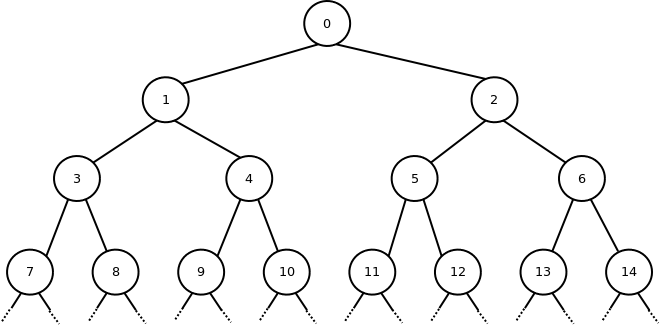
\includegraphics[width=\linewidth]{Kinfolk/fullTree.png}
\end{wrapfigure}

The integers identify the positions of person A and person B in a
family tree envisioned as follows: consider a full binary tree in
which the root is numbered 0, its children are numbered 1 and 2, and
numbering proceeds in that manner, level by level, left to right. This
numbering scheme is shown in the diagram to the right. A parent-child
relationship in this tree represents a parent-child relationship in
the family.


\subsection*{Output}

For each dataset, print a single line indicating the relationship of B
to A.  This relationship must be constructed from the phrases ``child'',
``parent'', ``niece'', ``nephew'', ``aunt'', ``uncle'', ``cousin'', ``grand'',
``great-'', ``1st'', ``2nd'', ``3rd'', ``once removed'', ``twice removed'', and
``thrice removed''.

\begin{itemize}
\item No more than two ``great-'' prefixes may be applied.

\item If  ``1st'', ``2nd'', or ``3rd'' is used, it should be separated from
  the following part of the line by a single blank.

\item If ``once removed'', ``twice removed'', or ``thrice removed'' is used,
  it must be separated from the preceding part of the line by a single
  blank.
\end{itemize}

If it is not possible to describe the relationship of B to A under the
above limitations, then print ``kin''.

\subsection*{Example}

Given the input:

\verbfile{Kinfolk/test0.in}


the output should be:

\verbfile{Kinfolk/test0.expected}




\clearpage
\problem{Of the Children}

\begin{quotation}
{\it This problem was withdrawn from the contest by a minute-1
clarification message sent to all teams.}

{\it The reason for the withdrawal was that, as of 24 hours before the
contest, the authoring team had only a single sample solution, and we
strongly prefer to move forward with a problem only after independent
confirmation by two or more authors.}
\end{quotation}

A nation-wide charity, {\em Won't Someone Think of the Children}, is
sending one of its celebrity spokespeople out on a coast-to-coast
publicity tour. Like many charities, they are bit strapped for funding
and need to plan carefully to make sure they can pay the celebrity's
travel expenses to get from their office on the west coast to the
final press event on the east coast.

Local offices of the charity have been taking pledges and collecting
donations to pay for this celebrity to visit their cities as part of
the tour. The national office has made no promises that the celebrity
will visit any of these intermediate locations, but hopes that these
locally collected funds can actually help fund the coast-to-coast
trip. In fact, without the help of the local offices, they aren't sure
they can afford to get their spokesperson to the final destination.

The trip will be paid for on an incremental basis. The celebrity can
only travel from one city to another if he or she has enough money to
pay for the transportation to that next city. Upon arrival at the
city, he or she can collect any money held there and use it to help
pay for the later legs of the journey. The celebrity can only visit a
given city once, lest multiple visits be considered an abuse of
their hospitality.

Given a list of cities that have invited the celebrity, the amount of
money raised by each city, and the travel costs between various pairs
of cities, what is the smallest amount of money that the home office
needs to provide the celebrity at the beginning of the journey to make
sure that he or she can make it all the way to the end without being
unable to pay for any leg of the trip?

\subsection*{Input}

Input will consist of one or more datasets. Each dataset begins with a
line containing a single integer, $N$, $2 \leq N < 24$, indicating the
number of cities involved. A value of zero for $N$ signals the end of
input.

Cities are identified by integers in the range $0\ldots N-1$, with
city $0$ being the home office and starting point of the journey, and
city $N-1$ being the final destination city for the journey.

The first line of the dataset is followed by $N-2$ lines, each
containing an integer in the range $0\ldots \num{10000}$ indicating the
amount of money collected by the cities numbered $1 \ldots N-2$. (The
amount of money at city $N-1$ is irrelevant and the amount of money to
be provided at city $0$ is what you need to compute).

This is followed by at least $1$ and up to $N(N-1)/2$ lines, each
containing three integers $i$, $j$, \& $c$.  $i$ and $j$ are distinct
integers in the range $0\ldots N-1$ identifying two cities and $c$ is
the cost to travel from one of those cities to the other, $0 < c <
\num{10000}$. The cost is the same when traveling from $i$ to $j$ as it is
when traveling from $j$ to $i$.  The end of this list of potential travel
expenses is indicated by a line containing negative values for $i$,
$j$, and $c$.


\subsection*{Output}

For each dataset print a single line of output. 

If it is possible to reach city $N-1$ from city $0$, print the
smallest amount of money that the celebrity needs to be given at city
$0$ in order to guarantee reaching city $N-1$.

If it is not possible to reach city $N-1$ when starting from city $0$, print $-1$.



\subsection*{Example}

Given the input:

\verbfile{OfTheChildren/test0.in}


the output should be:

\verbfile{OfTheChildren/test0.expected}




\clearpage
\problem{Talking About Numbers}

%\begin{wrapfigure}{r}{0.5\linewidth}
%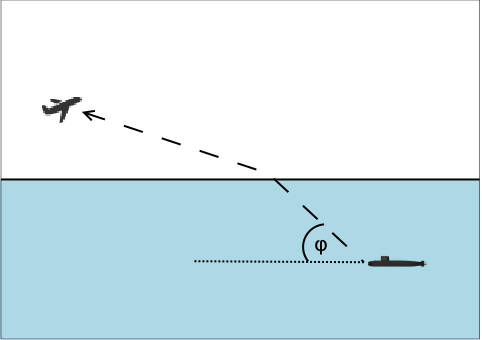
\includegraphics[width=\linewidth]{Refract/refract.png}
%\end{wrapfigure}

The programmers of a TTS (text-to-speech) program have discovered that
their product does a poor job of reading numbers written in
conventional numeric form. Currently, it just announces each digit in
the number, one after the other, which gets confusing to the listener
after a few digits have gone by.

They would prefer to have a more natural reading of numbers, and one
of them has suggested that, if they convert numeric strings into the
appropriate text equivalent, e.g., convert ``1023'' into ``one
thousand and twenty three'', then their speech engine will be able to
handle the reading with no further modification.

Write a program to carry out the transformation of non-negative
integers into conventional English wording:

\begin{itemize}

\item English has unique names for the numbers 0-19: ``zero'',
  ``one'', ``two'', ``three'', ``four'', ``five'', ``six'', ``seven'',
  ``eight'', ``nine'', ``ten'', ``eleven'', ``twelve'', ``thirteen'',
  ``fourteen'', ``fifteen'', ``sixteen'', ``seventeen'', ``eighteen'',
  ``nineteen''.

\item The subsequent multiples of 10 are named ``twenty'', ``thirty'',
  ``forty'', ``fifty'', ``sixty'', ``seventy'', ``eighty'', ``ninety''.

\item The combination of one of those multiples of ten with a digit
  1-9 is always hyphenated: e.g., $31 \Rightarrow$ ``thirty-one'', $77
  \Rightarrow$ ``seventy-seven''.

\item Multiples of 100 are counted 1-9 and set off from any following
  non-zero digits by 'and': e.g., $200 \Rightarrow$ ``two hundred'',
  $412 \Rightarrow$ ``four hundred and twelve'', $777 \Rightarrow$
  ``seven hundred and seventy-seven''.

\item Thousands and millions are counted off using the above rules to
  form numbers 1-999, and are set off from any non-zero remainder 
  by a comma: e.g., $\num{1253101} \Rightarrow$ ``one million, two hundred
  and fifty-three thousand, one hundred and one''.

\item If a number with a non-empty thousands or millions component is
  followed by a remainder of 1-99, then instead of a comma the parts
  are separated by ``and'': e.g., $\num{1000011} \Rightarrow$ ``one
  million and eleven'', $\num{20222043} \Rightarrow$ ``twenty million, two
  hundred and twenty-two thousand and forty-three''.
\end{itemize}

\subsection*{Input}

Input will consist of one or more datasets. Each dataset will consist
of a single line containing a non-negative integer in the range
$0\ldots \num{999999999}$. Although we have used commas within digit
strings for clarity in this problem description, there will be no
commas in the input. There will be no leading zeros on positive input
numbers.

A line with a negative value signals the end of input.

\subsection*{Output}

For each dataset, print a single line containing the spelled-out
equivalent of the number, according to the rules above.

Formatting requirements:
\begin{itemize}
\item The output must be left-justified.
\item All alphabetic characters must be in lower-case.
\item Exactly one blank must separate adjacent words, except when a
  hyphen or comma is called for.
\item When a comma is used, it must be followed by exactly one blank.
\item When a hyphen is used, no blank space appears to either side of
  the hyphen.
\end{itemize}


\subsection*{Example}

Given the input:

\verbfile{TalkingNumbers/test0.in}


the output should be:

\verbfile{TalkingNumbers/test0.expected}




\clearpage
\problem{The Scheming Gardener}

The Jackstraw Gardening Club is a cooperative of gardeners whose share
a common lot of land, parceling it out every year among their members,
each of whom gets their own plot of land within the larger lot.


Each winter, before the planting season, the club gathers together on
the lot to select their plots. Each member has a handful of wooden
stakes and a ball of string. Taking turns in rotation, each member may
choose to drive a new stake into the ground, and then may tie a length
of string between one or more pairs of stakes, forming a straight-line
connection between the two. Strings may not cross (except at the ends
where they are tied to same stake) nor may they lie directly atop one
another co-linearly. A string may not have both ends tied to the same
stake. Stakes may not be driven so close to an existing
string or stake that one could not easily step between them.

Each portion of the lot entirely surrounded by strings defines one
garden plot. The process continues until a majority of the club
members feel that enough enclosed plots have been formed, are willing
to stop, subject to the limitations:

\begin{itemize}

\item Upon stopping, any useless strings will be removed. A 
  useless string is one where the land just to each side of the string
  lies in the same plot or in the unenclosed portion of the lot.

\item At least one enclosed area must remain after removing the useless
  strings.

\item There will be no enclosed plots of zero area.

\item All the remaining strings (after the useless ones are removed)
  will be connected --- it will be possible to trace a path from one
  string to any other string in the lot.
\end{itemize}

The gardeners then choose their plots from among the enclosed areas.

\begin{wrapfigure}{r}{0.45\linewidth}
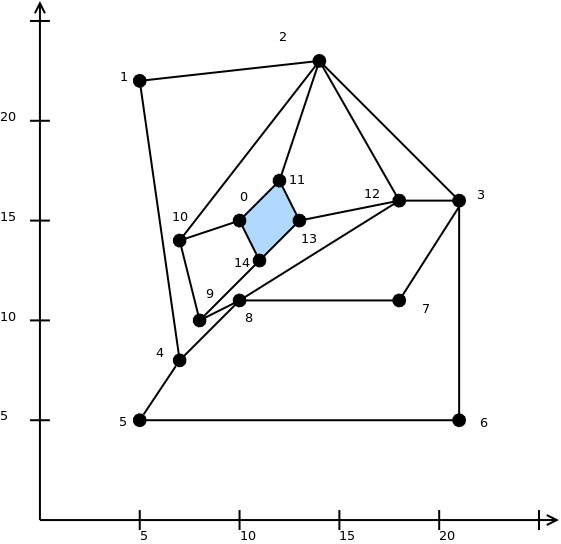
\includegraphics[width=\linewidth]{Gardener/plots1}
\end{wrapfigure}

You are lucky enough to have the first choice. You know that most of
your fellow gardeners will probably try for the largest area plots
they can get, but you have a different goal entirely. You are hoping
to raise a single, beautiful pumpkin that will win first prize at the
next county fair. You don't need much space, but you worry that your
pumpkins may be chewed upon by deer, rabbits, mice, and other
four-footed wildlife. You want to choose a plot that would force such
vermin to cross as many other plots as possible before reaching
yours. You hope that the sheer variety of crops presented by the other
gardeners will distract the vermin before they ever get to your plot. 
The vermin will not step directly on or over a stake, but will
always pass it to one side or the other.


\subsection*{Input}

Input will consist of 1 or more datasets.  Each dataset will begin
with a line containing two integers, $P$, and $E$. $2 < P \leq 750$, 
$3 \leq E \leq 1000$. A value of zero for $P$ indicates end of the input.

The first line of the dataset is followed by $P$ lines, each
containing $x,y$ coordinates of one point. These will be integers in the
range $0 \ldots \num{10000}$. These points will be distinct.

Those lines are followed by $E$ lines, each containing a pair of point
numbers, indicating a connection between those two points. These
numbers will be in the range $0\ldots P-1$ and refer to the order of
occurrence of the points in the earlier input, with point $0$ being the
first such point.


\subsection*{Output}

For each dataset, find a plot that maximizes the smallest number of
other plots that an animal approaching from outside would need to
cross before reaching your chosen one. Print the minimum number of
other plots that would need to be crossed by such an animal for your
chosen plot.


\subsection*{Example}


Here is a possible input:

\verbfile{Gardener/test0.in}


The output should be:

\verbfile{Gardener/test0.expected}


There are two datasets in the above input. The first, which ends with
the line containing ``0 14'', corresponds to the picture shown
above. The shaded plot in that picture is the one selected by the
scheming gardener.





\end{document}
